% Having presented ... ,
% the goal of this chapter is to demonstrate the use of the proposed query processing architecture in ...
% More specifically, we present case studies ...

% \section{Flexible secondary index partitioning}
% In section~\ref{sec:index_partitioning_background} we described the most common techniques for partitioning a secondary index:
% \begin{itemize}
%   \item \textbf{Partitioning by document}.
%   Each index partition is responsible for the data items of a corpus partition,
%   and is co-located in the same node as that corpus partition.
%   \item \textbf{Partitioning by term}.
%   Each index partition is responsible for a part of the \textit{value space} of the indexed attribute,
%   and its placement is independent from the corresponding corpus partition.
% \end{itemize}

% Experimental comparison of the two approaches has shown \cite{dsilva:tworings, kejriwal:slik} that there is no ``one-size-fits-all'' approach to secondary
% index partitioning.
% Rather, each approach caters to different needs.
% More specifically, partitioning by document is more suitable for:
% \begin{itemize}
%   \item Workloads with low selectivity queries, that return large result sets.
%   \item Corpora with skewed indexed attribute distributions (a large number of data items correspond to a few attribute values).
%   \item Write-intensive workloads that require low update latency.
% \end{itemize}
% \noindent
% On the other hand, partitioning by term is more suitable for:
% \begin{itemize}
%   \item Large-scale systems with a large number of corpus partitions.
%   \item High selectivity query workloads.
%   \item Corpora with normal indexed attribute distributions.
% \end{itemize}

% Therefore, the decision about which approach to be used for an index should be based on the corpus and the workload characteristics.

% In most existing system, the choice of index partitioning scheme is made during the system's design phase, and is therefore \textit{static}.
% For example, MongoDB \cite{coubase:mongoindexes}, Cassandra \cite{cassandra:secondaryindexing} and Riak \cite{riakv:secondaryindexes}
% use the partitioning by document approach,
% while HBase \cite{hbase:secondaryindexes} uses the partitioning by term approach.

% \bigskip
% \noindent
% In this section, we demonstrate the flexibility of QPU query processing architecture by showing how it can be used to
% express both index partitioning schemes.
% The design of the QPU architectures is based on observations about the properties of the alternative
% index partitioning schemes.
% We categorize these observations using the derived state read and write path framework presented in
% section~\ref{sec:read_write_path}:
% \begin{itemize}
%   \item In partitioning by document, the index \textbf{write path} is \textit{local}:
%   an index partition receives updates only from the corpus partition with which it is co-located.
%   On the hands, in partitioning by term, the write path involves a many-to-one relationship:
%   an index partition receives updates from all corpus partitions, corresponding to the value interval it is responsible for.

%   \item In partitioning by document, the \textbf{read path} is a \textit{broadcast} operation:
%   a query is forwarded to all index partitions.
%   On the other hand, in partitioning by term, only index partitions with relevant index terms are involved in processing a given query.
% \end{itemize}

% We present QPU architectures for the two index partitioning approaches using the photo album example of section~\ref{sec:read_write_path} as a reference.
% The corpus is composed of a set of image files, and each image can be associated with user-defined tags.
% The corpus is partitioned using a hash of the primary key as partitioning key.
% An application needs to create a secondary index on the $predominantColor$ tag, which can be assigned values in the range $[\#000000$, $\#FFFFFF$].

% Figures~\ref{fig:index_partitioned_by_document} and~\ref{fig:index_partitioned_by_term} show the QPU graphs and their
% placement across system nodes for a document-partitioned index and a term-partitioned index respectively.
% For simplicity we assume that the number of corpus partitions is equal to the number of system nodes,
% and that a corpus partition is placed on each node.

% In both architectures, an index QPU is used to represent each index partition;
% A partition manager QPU, connected to all index partitions, and is responsible for coordinating query access to them.
% Moreover, a corpus driver QPU is placed on each node, and is responsible for the data items of the corpus
% partition it is co-located with.

% \subsection{Write path}

% \begin{figure}
%   \begin{minipage}{.5\textwidth}
%     \centering
%     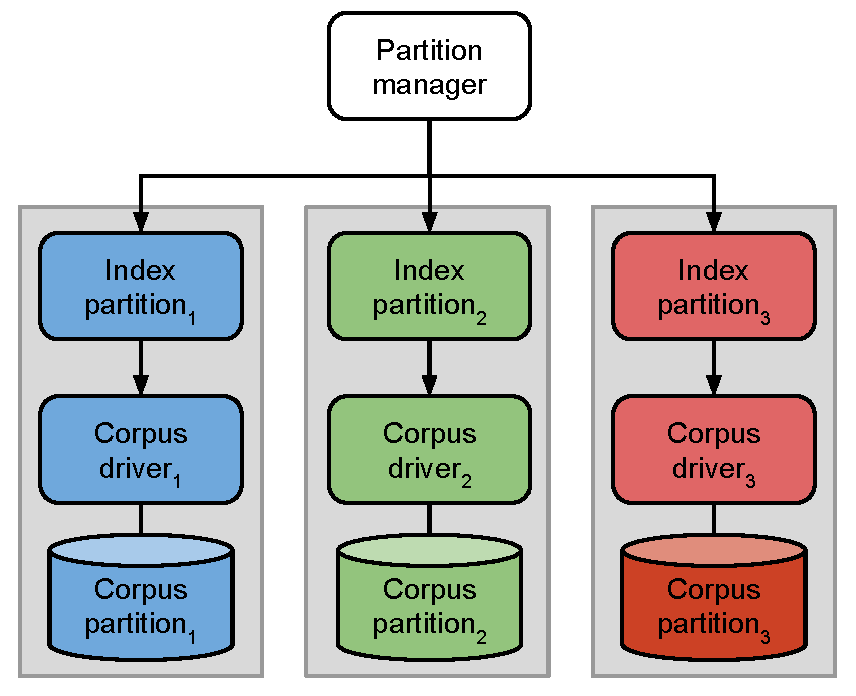
\includegraphics[scale=0.5]{./figures/case_studies/index_partitioned_by_document.pdf}
%     \caption{QPU architecture for a document-partitioned secondary index.}
%     \label{fig:index_partitioned_by_document}
%   \end{minipage}%
%   \begin{minipage}{.5\textwidth}
%     \centering
%     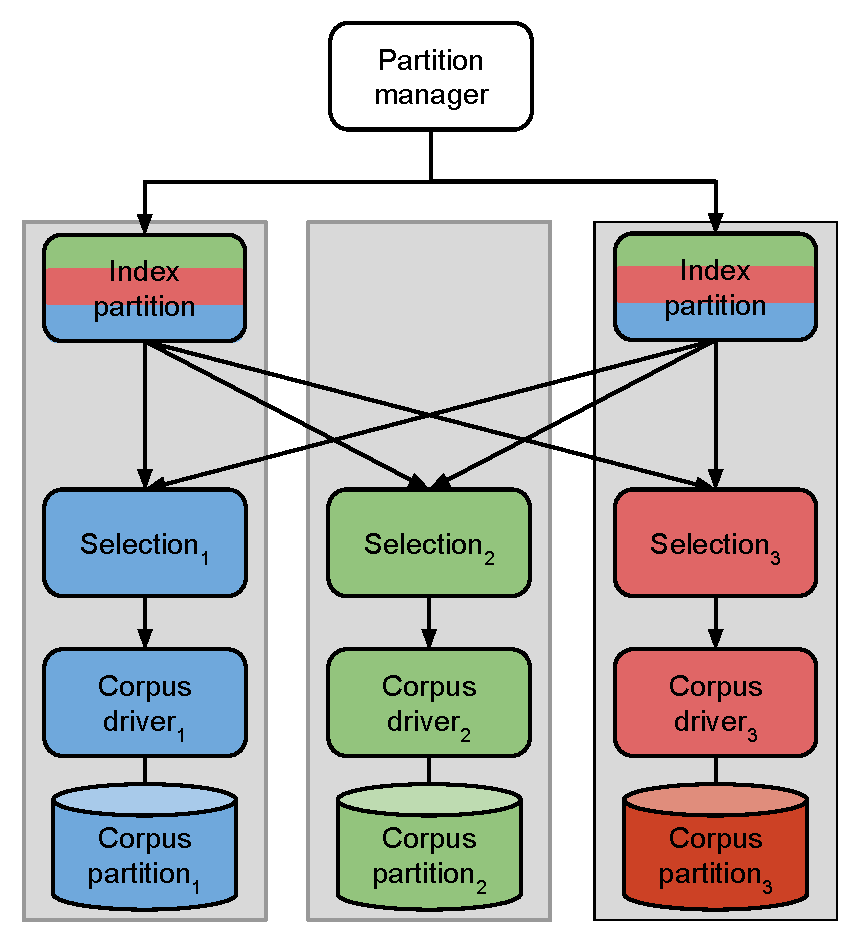
\includegraphics[scale=0.5]{./figures/case_studies/index_partitioned_by_term.pdf}
%     \caption{QPU architecture for a term-partitioned secondary index.}
%     \label{fig:index_partitioned_by_term}
%   \end{minipage}
% \end{figure}

% The write path properties described above are achieved through (1) the QPU graph topology and the placement of graph vertices across system nodes,
% and (2) the configuration of the index QPUs (index partitions).

% \subsubsection{Graph topology and placement}

% \medskip
% \noindent
% \textbf{Partitioning by document.}
% In the partitioning by document approach, an index partition is placed on each system node, and is connected to the
% corresponding corpus driver.
% Therefore, each index partition communicates only with the corpus driver it is co-located with.

% \medskip
% \noindent
% \textbf{Partitioning by term.}
% In the partitioning by term approach, index partitions can be flexibly placed across nodes.
% Each index partition is connected to all corpus driver QPUs, because an index partition is responsible for data
% items in all corpus partitions.
% Moreover, a filter QPU is connected to each corpus driver.
% This permits each update to be forwarded to the relevant index partition based on the attribute value in the update.

% \subsubsection{Index partition configuration and graph initialization}

% When the QPU graph for one of the partitioned index architectures is initialized,
% the initialization function of each index partition sends interval queries to the QPU's downstream connections,
% in order to establish an input stream of updates.
% The initialization function uses the index QPU's \textit{configuration} to generate the appropriate query request for each
% downstream connection.
% More specifically, each index QPU is configured with an attribute ($predominantColor$ in this example),
% and an \textit{interval of values} of that attribute.
% The index partition is responsible for index entries that correspond to attribute values in the specified interval.

% \medskip
% \noindent
% In the partitioning by document approach,
% all index partitions are configured to be responsible for the entire attribute value space,
% which in the photo album example is $[\#000000$, $\#FFFFFF$].
% Conversely, in the partitioning by term approach, each index partition is responsible for a non-overlapping subset of the
% attribute value space.
% A simplified version of the configuration of the index partitions of the term-partitioned index QPU architecture
% (figure~\ref{fig:index_partitioned_by_term}) is depicted below: \\

% \noindent\begin{minipage}{.48\textwidth}
% \begin{lstlisting}[caption={Configuration of $index_1$ in Figure~\ref{fig:index_partitioned_by_term}},captionpos=b,frame=tlrb]{Name}
% {
%   // other configuration
%   // parameters
%   "indexConfiguration": {
%     "table": "photoAlbum",
%     "attribute":
%         "predominantColor",
%     "lower_bound": #000000,
%     "upper_bound": #7FFFFF
%   }
% }
% \end{lstlisting}
% \end{minipage}\hfill
% \begin{minipage}{.48\textwidth}
% \begin{lstlisting}[caption={Configuration of $index_2$ in Figure~\ref{fig:index_partitioned_by_term}},captionpos=b,frame=tlrb]{Name}
% {
%   // other configuration
%   // parameters
%   "indexConfiguration": {
%     "table": "photoAlbum",
%     "attribute":
%         "predominantColor",
%     "lower_bound": #7FFFFF,
%     "upper_bound": #FFFFFF
%   }
% }
% \end{lstlisting}
% \end{minipage}

% \noindent
% In the case of the document partitioned index architecture, all index partitions have the same ``indexConfiguration'' with
% $lower_bound$ $=$ $\#000000$ and $higher_bound$ $=$ $\#FFFFFF$.
% Therefore, in the \textbf{document-partitioned} index architecture, upon initialization, each index partition sends the query \\
% {\obeylines\obeyspaces
%   SELECT primaryKey, predominantColor
%   FROM photoAlbum
%   INTERVAL FROM LATEST
% } ~\\
% to the corpus driver it is connected to.
% This establishes a stream between each corpus driver and the corresponding index QPU, through which the corpus driver
% sends to the index QPU notifications for updates to the data item of the corpus partition it responsible for,
% which the required read path behavior for the document-partitioned index.

% \medskip
% \noindent
% In the \textbf{term-partitioned} index architecture, upon initialization, $index_1$ sends the query \\
% {\obeylines\obeyspaces
%     SELECT primaryKey, predominantColor
%     FROM photoAlbum
%     WHERE predominantColor $\geq$ $\#000000$ AND predominantColor $<$ $\#7FFFFF$
%     INTERVAL FROM LATEST
% } ~\\
% to each filter QPU it is connected to, and $index_2$ \\
% {\obeylines\obeyspaces
%   SELECT primaryKey, predominantColor
%   FROM photoAlbum
%   WHERE predominantColor $\geq$ $\#7FFFFF$ AND predominantColor $leq$ $\#FFFFFF$
%   INTERVAL FROM LATEST
% } ~\\
% to each of its downstream connections.

% \noindent
% Each filter QPU in turn establishes for each received query, an input stream of data item from the corpus partition it
% is connected to, by sending the query: \\
% {\obeylines\obeyspaces
%   SELECT primaryKey, predominantColor
%   FROM photoAlbum
%   INTERVAL FROM LATEST
% } ~\\
% As a result, updates on data items of each corpus partition are sent from the corpus driver to the filter QPU corresponding
% to that partition.
% The filter QPU forwards each update to the corresponding index partition, based on the attribute value in the update.
% This achieves the required write path functionality for the term-partitioned index.

% For example, as a result of the creation of an image file with $predominantColor$ $=$ $\#613930$, assigned to to $corpus$
% $partition_2$, $corpus$ $driver_2$ sends to $filter_2$ a record encoding that update.
% This input record matches the query \\
% {\obeylines\obeyspaces
%     SELECT primaryKey, predominantColor
%     FROM photoAlbum
%     WHERE predominantColor $geq$ $\#000000$ AND predominantColor $<$ $\#7FFFFF$
%     INTERVAL FROM LATEST
% } ~\\
% and thus the filter QPU sends the update record only to the $index_1$ partition.


% \subsection{Read path}
% In both QPU architectures, the partition manager QPU is connected to all index partitions.
% As described in section~\ref{sec:qpc_tree}, given a query,
% the partition manager's query processing function determines which index partitions need to be contacted and generates
% the corresponding queries, using the query processing capabilities trees of its downstream connections.

% More specifically, the query processing function, performs an ``intersection'' between the query parse tree
% and the QPC tree of each of its downstream connections.
% The result of each intersection operation is a query parse tree representing the downstream query that the partition manager
% needs to send to the corresponding index QPU.
% If the intersection result is empty, then no query needs to be sent by the partition manager to the corresponding
% connection.

% \begin{figure}
%   \centering
%     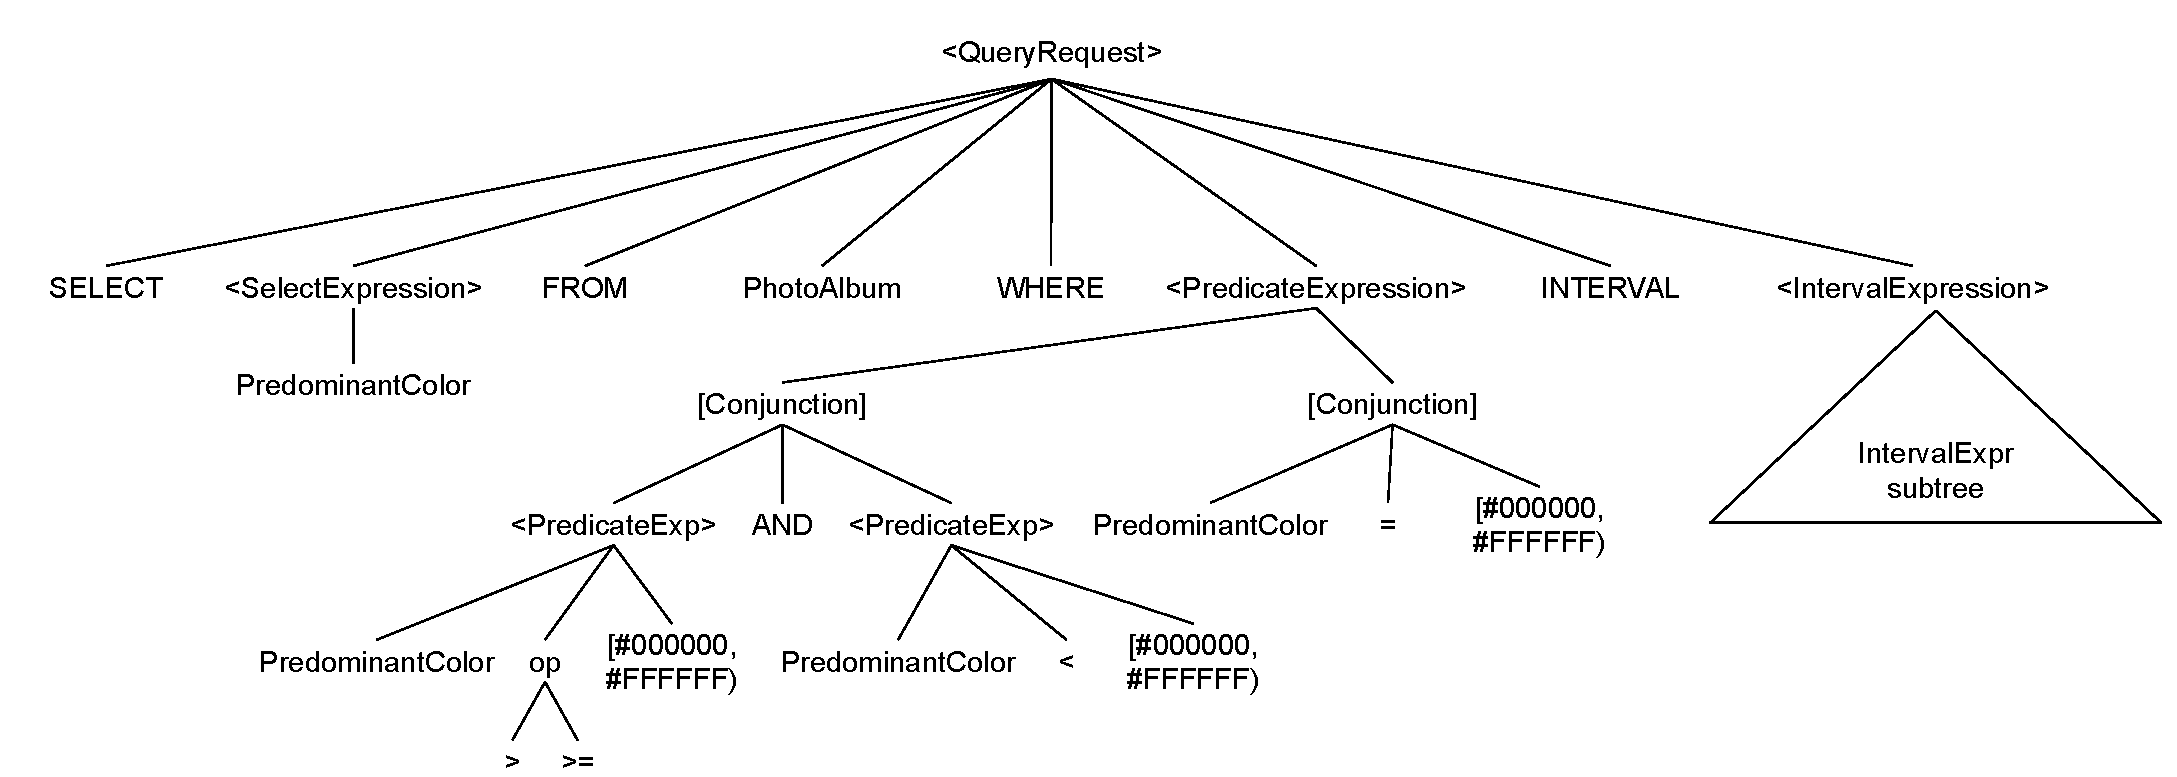
\includegraphics[width=\textwidth]{./figures/case_studies/qpt_index_partitioning_docs.pdf}
%   \caption{Query processing tree of an index partition in the document-partitioned index QPU architecture.}
%   \label{fig:qpt_index_partitioning_docs}
% \end{figure}

% \medskip
% \noindent
% \textbf{Partitioning by document}
% The QPC tree for an index partition in the document-partitioned index QPU architecture is shown in Figure~\ref{fig:qpt_index_partitioning_docs}.
% As describe above, in the document-partitioned index each index partition is responsible for the entire attribute value space of
% for the data items of one corpus partition.
% The QPC tree for all index partitions thus  are the same.
% Moreover, because this tree corresponds to the entire attribute value domain, the intersection with any query parse tree
% is an identity function:
% the result is the same parse tree as that of the received query.
% As a result, the partition manager forwards each received query to all index partitions,
% which is the required write path behavior.

% \begin{figure}
% % \subfloat[]{%
% % \centering
% %   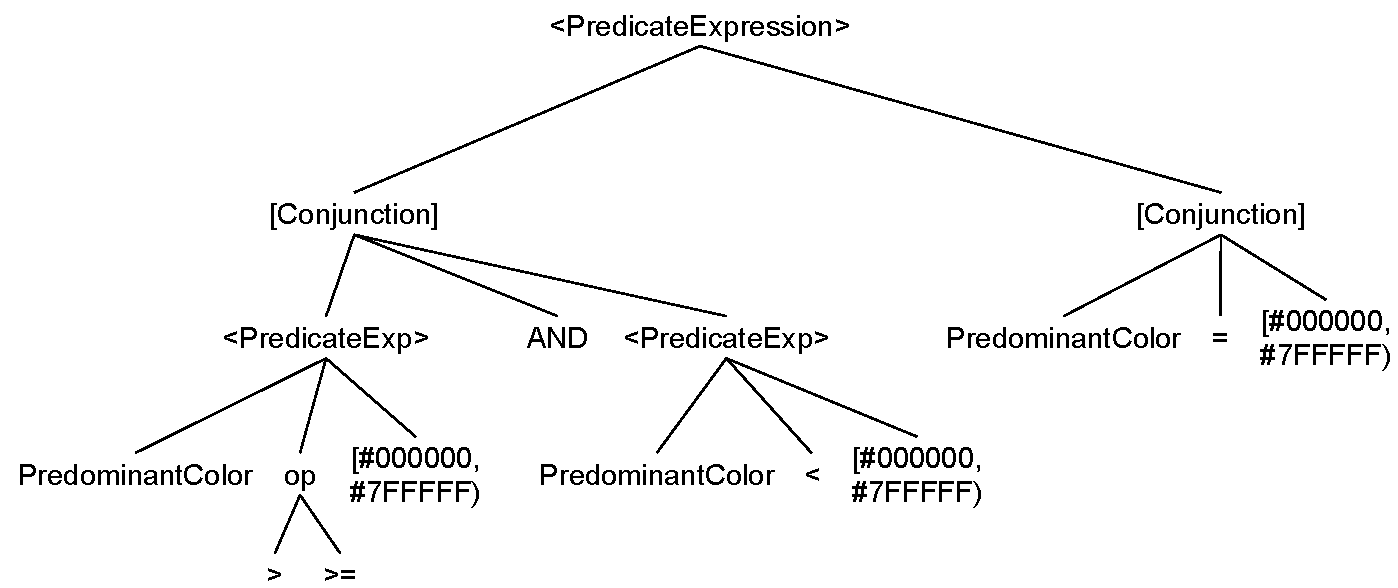
\includegraphics[width=\textwidth]{./figures/case_studies/qpt_index_partitioning_terms_1.pdf}%
% % }

% % \subfloat[]{%
% %   \centering
% %   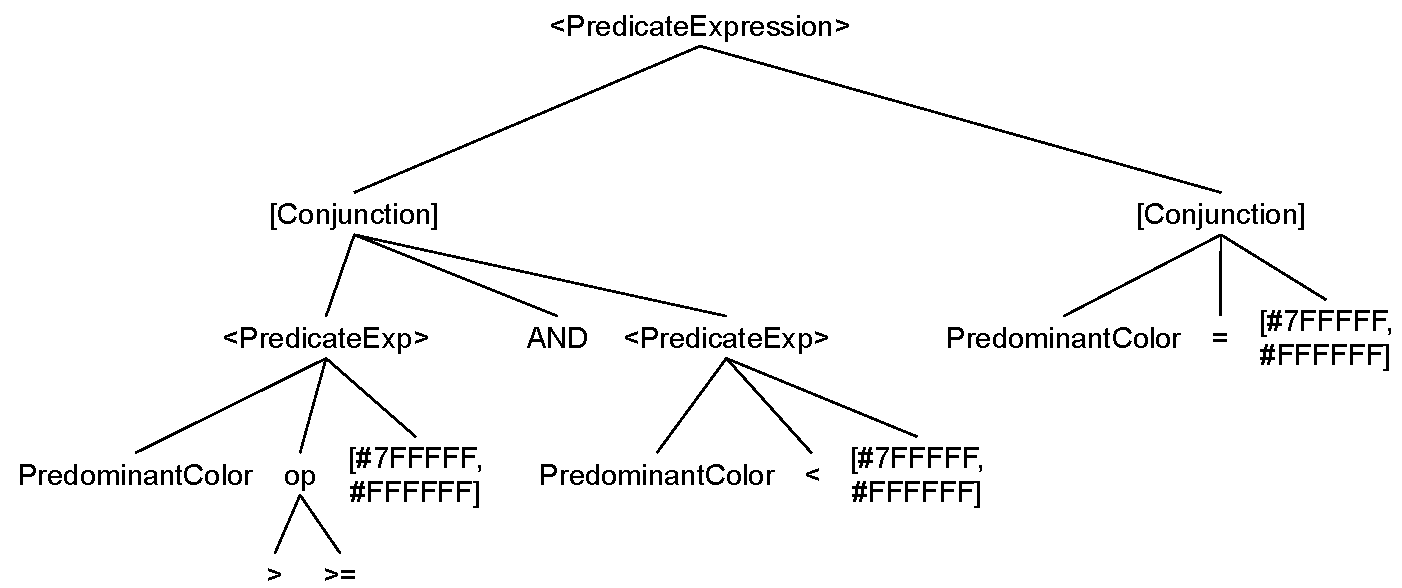
\includegraphics[width=\textwidth]{./figures/case_studies/qpt_index_partitioning_terms_2.pdf}%
% % }
% % \caption{The query processing capabilities tree for index partitions $index_1$ (a) and $index_2$ (b) of the term-partitioned
% % index in Figure~\ref{fig:index_partitioned_by_term}}
% \label{fig:qpt_index_partitioning_terms}
% \end{figure}

% \medskip
% \noindent
% \textbf{Partitioning by term}
% Figure~\ref{fig:qpt_index_partitioning_terms} shows the $<predicateExpression>$ subtrees of the QPC tree for $index_1$ and $index_2$ in the term-partitioned index QPU
% architecture.
% The QPC tree of $index_1$ represents the set of queries in the $[\#000000$, $\#7FFFFF$) interval,
% while the QPC tree of $index_2$ represents the interval $[\#7FFFFF$, $\#FFFFFF$].

% Given the query \\
% {\obeylines\obeyspaces
% Q = SELECT primaryKey, predominantColor
%     FROM photoAlbum
%     WHERE predominantColor $\geq$ $\#21B1FF$ AND predominantColor $<$ $\#ff7b75$
%     INTERVAL FROM LATEST
% } ~\\
% the intersection between the parse tree of $Q$ the QPC tree of $index_1$ results to the query \\
% {\obeylines\obeyspaces
% Q1 = SELECT primaryKey, predominantColor
%     FROM photoAlbum
%     WHERE predominantColor $\geq$ $\#21B1FF$ AND predominantColor $<$ $\#7FFFFF$
%     INTERVAL FROM LATEST
% } ~\\
% and the intersection between the parse tree of $Q$ the QPC tree of $index_2$ results to the query \\
% {\obeylines\obeyspaces
% Q2 = SELECT primaryKey, predominantColor
%     FROM photoAlbum
%     WHERE predominantColor $\geq$ $\#800000$ AND predominantColor $<$ $\#ff7b75$
%     INTERVAL FROM LATEST
% } ~\\
% The partition sends a query request for Q1 to $index_1$ and Q2 to $index_2$.
% It merges the returned streams and emits the merged stream as its output stream.

% In summary, in the term-partitioned index QPU architecture,
% for a given query, the partition manager generates and sends downstream queries to index partitions according their corresponding
% value intervals, using the QPC tree mechanism.

% \medskip
% \noindent

% Using ... [basically say that the value here is to support select the partitioning scheme during index creation]

% It is important to note that DynamoDB \cite{dynamodb:secondaryindexes} and Apache Phoenix \cite{phoenix:secondaryidnexing}
% support index partitioning schemes.
% However, we believe that the proposed framework provides a more structured approach to the design of query processing system.

% Furthermore, the proposed approach is more flexible, as it enables 



% \section{Federated attribute search in multi-cloud object storage}

% \section{Materialized views at the edge}
% % \section{Scalability middleware pushing materialized view to the edge}

% % news aggregator application

% % Lobsters stores individual votes for stories in a votes ta- ble, but also stores per-story vote counts as a column in the stories table. This speeds up read queries of vote counts, but “de-normalizes” the schema and complicates vote writes, which must update the derived counts.
% % CREATE TABLE stories (id int, author int, title text, url text);
% % CREATE TABLE votes (user int, story_id int);
% % CREATE TABLE users (id int, username text);

% % CREATE INTERNAL VIEW VoteCount AS
% % SELECT story_id, COUNT(*) AS vcount
% % FROM votes GROUP BY story_id;

% % CREATE VIEW StoriesWithVC AS
% % SELECT id, author, title, url, vcount
% % FROM stories
% % JOIN VoteCount ON VoteCount.story_id = stories.id
% % WHERE stories.id = ?;



% \bibliographystyle{plainnat}
% \bibliography{refs}